% TODO: CITACAO DEPOIS DO CONCEITO
In the context of our research, we consider classes as the components

\section{Abstract}

Software modularization recovery algorithms automatically recognize a system's
modular structure by analyzing its implementation.
Due to the lack of well document software systems, though, the issue of testing
these algorithms is still underexplored, limiting both their adoption in the
industry and the development of better algorithms.
We propose to rely on software models to produce arbitrarily large test sets. In
this paper we consider three such models and analyze how similar the artifacts
they produce are from artifacts from real software systems.
\cite{Pollet2007}

\section{Introduction}

Development of large-scale software systems is a challenge.

A key to success is the ability to decompose a system into weakly-coupled
modules, so each module can be developed by a distinct team. Failing to do so
results in duplicated code, non-parallelism, one's work impacting another's work
etc.

The ability do modularize depends decisively on a vast knowledge about the
system, how its different parts interact to accomplish the system's goal.

Unfortunately, in the case of legacy systems, such knowledge isn't available.
Depending on its size, it might take months to understand the system so well as
to find a good modularization. XXX \cite{Parnas1972}

POR ISSO SURGIRAM software modularization recovery algorithms, also known as
software clustering algorithms or software architecture recovery algorithms. In
its most common flavor, these algorithms analyze the dependencies between
implementation components, such as classes, and then group them into modules
such as there are few dependencies between classes in distinct modules.

Software modularization recovery algorithms can, therefore, do in minutes what a
person would spend weeks or months. The question is: are the found
modularizations good? Are they similar to what a person would find? To answer
this question it's essencial to perform empirical evaluations envolving systems
with known reference modularizations.

The empirical evaluations consist of selecting a collection of systems with
known reference modularizations and then applying the algorithms to the systems.
The modularizations found by the algorithms are then compared to the reference
decompositions by a metric such as MoJo \cite{Tzerpos1999} or PrecisionRecall.

  \begin{figure*}[!t]
  \centering
  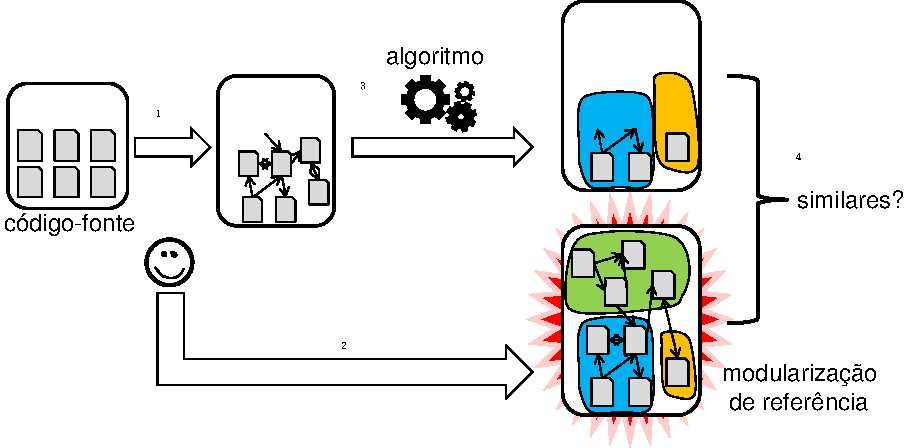
\includegraphics[width=1.0\textwidth]{diagram}
  \caption{Evaluation of a software modularization recovery algorithm}
  \label{fig:diagram}
  \end{figure*}

% TODO: diagram showing the evaluation of a clustering algorithm

Unfortunately there are few systems with known reference modularizations and,
because to obtain reference modularizations is costly, there are few empirical
studies, and most of them consider a couple of small and medium systems.

We therefore propose to use synthetic, i.e., computer-generated, software
dependency networks, to evaluate software modularization recovery algorithms.
These networks are generated by parametrizable models and have an embedded
reference modularizations. The goal of an algorithm is, thus, to find
modularizations that are similar to the reference modularization embedded in the
network. With this approach we can CONTAR COM a large volume of test data that
is composed of networks of different sizes and controllable characteristics.

Of course the success of this approach depends on the realism of the synthetic
networks, ie, how well they resemble networks extracted from real software
systems. In this paper we study three models and show that all of them are, by
means of a careful parameter choosing, capable of producing realistic software
networks.

The remaining sections are organized as follows. .... Section 2, ...

%alike, resembling, exchangeable, indistiguible

\section{Related Work}

\section{Software Modularization Recovery: an Overview}

Aka software architecture recovery, software architecture reconstruction,
software clustering...

It's an task of reverse engineering, as defined by Tonella \cite{Tonella2007}...

DEFINITIONS

external edge...

%\section{Software Networks and Software Clustering}

directed graph, (un)weighted

\section{Network Theory}

Network theory research studies general properties of many types of networks by
using statistical analysis. In the last decade, it has been found that many
networks arising from sociology, biology, technology and other domains present
remarkable structural similarities. It has been shown that, in these networks,
the number of vertices connected to k edges, N(k), is proportional to
$k^{\-gamma}$, where $\gamma$ is a positive constant. These networks were called
scale-free networks.

Network theory has been applied to software networks and it was shown that they
are also scale-free networks \cite{Myers2003,Valverde2003}.

(in fact we can't argue the degree distribution is perfectly fit by a power law.
Anyway, the distribution is much more assymetric than normal ou Poisson's)

software indegree distribution (power law), outdegree distribution (not so power
law)

\section{Network Models}

Many models were proposed to explain the formation of scale-free networks. These
models are simple algorithms that can be proven, either formally or empirically,
to generate networks that are scale-free. In this section we present three
models that generate directed networks with built-in modular decomposition:
BCR+, CGW and LR. The first two models grow networks using a mechanism called
preferential attachment CITE Barabasi, by which nodes with many edges tend to
receive more edges in the process.

%\subsection{ER (Erdos-Renyi)}

%\subsection{Configuration model}
% take the most typical software system and steal its degree sequence

\subsection{BCR plus}

The BCR model aims to model the network of hyperlinks between web pages as a
directed graph without modules \cite{Bollobas2003}. It was proven analitically
to generate scale-free networks. We have developed an extension to this model,
which we will call BCR+, that adds the concept of module. The model accepts the
following parameters:

\begin{itemize}
\item number of vertices, $n$;
\item a graph, $G$;
\item three probabilities, $p$, $q$, and $r$, such as $p + q + r = 1$;
\item a probability, $mu$;
\item two real numbers, din and dout.
\end{itemize}

In a network with modules, one can define a MDG as a graph where the two
following conditions hold:
* each vertex represents a module in the original network;
* there is an edge from M1 to M2 in the MDG only if there is an edge from 
v1 to v2 in the original network, where v1 in M1 and v2 in M2.

The BCR+ model generates networks whose MDG is equal to G by adding vertices and
edges to an initial network until it reaches n vertices. The initial network is
isomorphic to G: it contains one vertex for each module and one edge for each
edge in G, connecting vertices whose corresponding modules are are connected.
Thus, the networks's MDG is equal to G from the very beginning.

After that, the algorithm consists of successive applications of one out of
three operations on the network: (1) adding a vertex with an outgoing edge; (2)
adding a vertex with an ingoing edge; (3) adding a edge between existing
vertices. The choice of the vertices that will be connected by a new edge,
although non-deterministic, is not fully random. The probability that a
particular vertex v is choosen, P(v), is proportional to a function of the
in-degree or of the out-degree of the node. We say that we choose a vertex
within a set V according to a function f if

  P(choose v) = f(v) / sum(v in V, f(v))

The denominator is a normalizing factor that assures that the probabilities sum
to 1.

Before we present the algorithm in detail, using pseudo-code, we must explain
some definitions. V is the set of vertices in the network being generated. This
set grows as the algorithm is executed. Being v a vertex, we define the
following three functions:

* out-neighbors(v): the set of all vertices that are connected to v by an edge
starting in v.
* same-module(v): the set of all vertices that are in the same module as v (except
v itself).
* other\_modules(v): the set of all vertices that are in modules that are connected
to v's module (in the graph G) by an edge starting in v's module.

After the initial network is created, the algorithm proceeds as follows:

while the network has less than n vertices:
  choose one of the operations according to probabilities (p, q, r)
  operation 1: (add a vertex with an outgoing edge)
    choose a vertex w within V according to f(x) = din + in-degree(x)
    add a new vertex v to w's module
    add an edge from v to w
  operation 2: (add a vertex with an ingoing edge)
    choose a vertex w within V according to f(x) = dout + out-degree(x)
    add a new vertex v to w's module
    add an edge from w to v
  operation 3: (add an edge between two existing vertices)
    choose a vertex v within V according to f(x) = dout + out-degree(x)
    choose a case according to probabilities (mu, 1 - mu)
    case 1: (distinct modules)
  	choose a vertex w within (other\_modules(v) - neighbors(v)) according to f(x) = din + in-degree(x)
      add an edge from v to w
    case 2: (same module)
      choose w within (same-module(v) - neighbors(v)) according to f(x) = din + in-degree(x)
      add an edge from v to w
  end

We can see that the probabilities p, q and r control how often each operation is
performed. Because the operation associated with probability r does not add any
vertices, greater values of r imply more edges in the resulting network. It is
easy to see that nodes connected to many ingoing edges are more likely to get
another ingoing edge, and the same reasoning can be applied to outgoing edges.
The parameter din can alleviate the handicap by providing a ``base in-degree''
that is applied to all vertices when computing the probabilities. Consider
two vertices, v1 with in-degree 4, and v2 with in-degree 8. If din = 0, v2 is
twice more likely to receive a new incoming edge; if, otherwise, din = 4, v2 is
only 3/2 more likely to receive the edge.

The parameter mu controls the proportion of edges between vertices in distinct
modules. Lower values of mu lend to networks that are more modular.

The BCR+ model is a growth model, meaning that the network is generated vertex
by vertex, growing from an initial network. It can, therefore, simulate the
evolution of a software network. Moreover, it can simulate the evolution of a
software system subject to constraints in module interaction, as is the case
with top-down design methodologies CITE.

%* Add a node with ongoing edge. With probability p, a new vertex is added to the network, together with an
%edge from the new vertex to an existing vertex, chosen preferentially according
%to .... Considering din = 0, this means that a vertex with indegree = 8 is
%twice more likely to receive the edge than a vertex with indegree = 4. The
%parameter din can be used to alleviate the handicap. (If din = 4, the first
%vertex will only be 3/2 more likely to receive the edge). The new vertex is
%put on the same cluster as the old vertex.
%
%* Add a node with ingoing edge. With probability q, a new vertex is added to the network, together with an
%edge from an existing vertex, chosen preferentially accordingly to dout +
%outdegree, to the new vertex. The new vertex is put on the same cluster as the
%old vertex. This case is similar to the previous case.
%
%* Add an edge. With probability r, a new edge is added between two vertices, v and w. v is
%chosen according to .... After that, with prob X, w is chosen from one of the
%modules connected to v's module, else it's chosen from v's own module. In any
%case, the exact choice is made according to ...
%
%It's a growth model, that is, it can take as input an existing network and
%evolve it.
%
%TODO: Argument: why the imposed modules are natural modules?

\subsection{CGW}

The CGW model was proposed to model the evolution of software systems organized in
modules. It was proven formally to generate scale-free networks. \cite{Chen2008}
It accepts the following parameters:

* n, m
* Probabilities p1, p2, p3, p4, summing 1
* Natural numbers e1, e2, e3, e4
* alpha

Just like BCR+, this is a growth model. Its initial network is composed of two
vertices belonging to the same module and a directed edge between them. The
remaining m - 1 modules are initially empty. Because the original implementation
of the model is not available, we describe in detail the algorithm we
implemented:

while the network has less than n vertices:
  choose operation (p1, p2, p3, p4)
  operation 1: (adding a vertex with e1 edges)
    create a new vertex v and add it to a randomly chosen module
    do e1 times:
      choose a vertex w according to mbpa(v)
      add an edge from v to w
  operation 2: (adding e2 edges)
    do e2 times:
      choose a vertex v randomly
      choose a vertex w according to mbpa(v)
      add edge from v to w
  operation 3: (rewiring e3 edges)
    do e3 times:
      choose a vertex v randomly
      choose an edge e randomly within edges that start in v
      choose w according to mbpa(v)
      remove e
      add an edge from v to w
  operation 3: (removing e4 edges)
    do e4 times:
      remove and randomly chosen edge
    

Unlike BCR+, this model does not allow constraints on the connection between
modules, however it accounts for the rewiring and the removal of edges. 

\subsection{LF}

The LF model is a very flexible model that can generated weighted directed
networks with overlapping modules, that is, in which a vertex can belong to more
than one module. Unlike the previous models, this is not a growth model: all
vertices are generated at once and then the edges are added.

There is also a special version of the model in which the edges weights are
discarded and the modules are non overlapping. We used the original
implementation of this version, available at http://. 

%%%%%%%%%%%%%%%%%%%%%%%%%%%%%%%%%%%%%%%%%%%%%%%%%%%%%%%%%%%%%%%%%%%%%%%%%%%%%%
%%%%%%%%%%%%%%%%%%%%%%%%%%%%%%%%%%%%%%%%%%%%%%%%%%%%%%%%%%%%%%%%%%%%%%%%%%%%%%
%%%%%%%%%%%%%%%%%%%%%%%%%%%%%%%%%%%%%%%%%%%%%%%%%%%%%%%%%%%%%%%%%%%%%%%%%%%%%%

\section{Characterization of Software Networks}

Our research hypothesis is that at least one of the presented models can
synthesize networks that resemble software networks. A central issue, thus, is
how to measure similarity between networks. In order to be useful, the metric
must be able to differentiate between software and non-software networks. In
this section we present such a metric, together with an experiment that
evaluates its usefulness by applying it to both software and non-software
networks. %Then we show a classification model 

\subsection{Similarity Between Networks}

In a recent work, Milo et al. \cite{Milo2002} proposed to characterize networks
by analyzing their triad concentration. A triad is a network with three vertices
in which all vertices are connected. There are only 13 distinct triads, one for
each configuration of directed edges, as shown in Figure \ref{fig:triads}.

\begin{figure*}[!t]
\centering
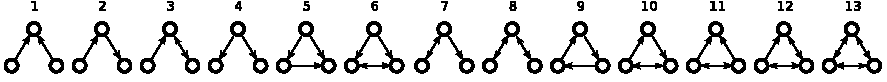
\includegraphics[width=1.0\textwidth]{triads}
\caption{Triads (id vs. graph. reprs.)}
\label{fig:triads}
\end{figure*}

By counting how many times each triad appears in a network, one can build a
triad concentration profile (TCP), which is a vector with 13 numbers that
summarize the local structure of the network. Figure \ref{fig:profiles} shows
the TCP for three distinct networks.

Following the work by Milo et al. \cite{Milo2002}, similarity between two
networks can be measured by computing Pearson's correlation coefficient between
the corresponding TCPs, which yields a value between -1 (most dissimilar) and 1
(most similar):

$$
\mathrm{sim}(a, b) ~=~ \mathrm{cor}(\mathrm{TCP}(a), \mathrm{TCP}(b))\mathrm{,}
$$

where $a$ and $b$ are networks, TCP($x$) is the triad concentration profile for
network $x$, and cor($x$, $y$) is Pearson's correlation coefficient.

\begin{figure*}[!t]
\center
\subfigure[ref1][Software
network]{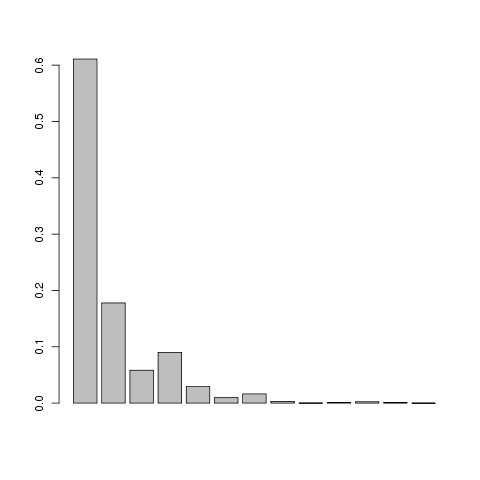
\includegraphics[width=2.5in]{triads-software}}
\hfil
\subfigure[ref2][Non-software network]{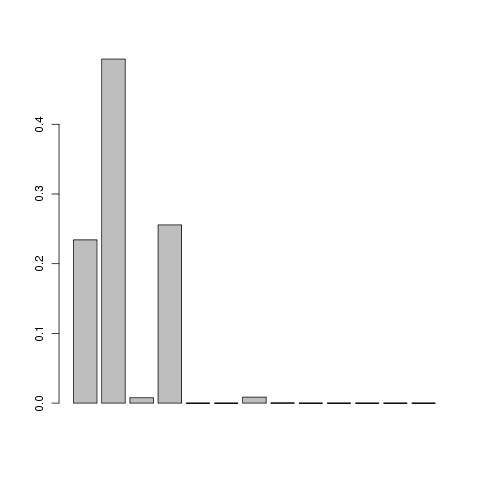
\includegraphics[width=2.5in]{triads-nonsw}%
}
\caption{Triad profiles}
\label{fig:profiles}
\end{figure*}

\subsection{Data Set}

To support the evaluation of the metric, we have collected 131 networks. The
networks are described in detail in Appendix A.

\textbf{Software networks}. We have collected 65 software systems written in
Java, with size ranging from 111 to 35,363 classes. Java was chosen for being a
popular programming language in which many open source systems have been
written. The software networks, representing dependencies between classes, were
extracted with the tool Dependency Finder CITE.

\textbf{Non-software networks}. We have collected 66 networks from distinct
domains, such as biology, sociology, technology, and linguistics. These networks
are freely available on the Internet and have been used in previous researches.

% S-score

\subsection{Evaluation of the Similarity Metric}

In order to evaluate the similarity metric, we measured the similarity between
the networks in the data set. A suitable metric must fullfil two conditions: (i)
it must yield high similarity between software networks, and (ii) it must yield
lower similarity between software networks and networks from other domains.

Using the data set we can define S-score, a metric that represents how much a
particular network resemble software networks. It is defined as the average
similarity between the network and a sample of software networks:

$$
\mathrm{S\mbox{-}score}(a) = \frac{
\sum_{s \in S} cor(a, s)
}{|S|} \mathrm{,}
$$

where $S$ is the set of sample software networks, and $|S|$ is the cardinality
of $S$. In this work we use the full software data set consisting of 65 software
networks.

We measured the S-score for each software network, which ranged from 0.83 to
0.98. The average S-score was 0.97 and the standard deviation, 0.03. The high
average S-score and the low standard deviation show that the metric successfully
captures common structural patterns in software networks.

TODO: Boxplot by network class (software, metabolic, neural, social etc.)

Then we measured the S-score for each non-software network. The majority of the
networks (X\%) have a S-score lower than 0.83, which shows that they
are ... Networks extracted from the social network Facebook have negative
S-score.

A few networks, though, showed high S-score. The network
polblogs, showing links between blogs on politics, had similarity 0.97. The
neural network of C Elegans also had a high similarity (0.88). Further
investigation is needed in order to discover why does it happen and whether
auxiliary metrics can differentiate these networks from software networks.

\subsection{A Network Classification Model}

Although the S-score of a network tells how close it is from software networks,
it does not tell whether a network is close enough that it can be considered
software-like. What is needed is a binary classification model that
distinguishes software-like networks from the other networks. The distinction
can be made by choosing a suitable S-score threshold. Networks with S-score
below the threshold are considered dissimilar from software networks; only
networks with S-score above the threshold are considered software-like. 

As we have shown on the previous section, there are non-software networks with
high S-scores, hence it is impossible to build a perfect classification model,
regardless of the threshold. Nonetheless, such a model can be evaluated by its
precision and recall. Consider a data set with both software and non-software
networks. Let $S$ be the set of all software networks, and $L$ the set of all
networks that were classified as software-like. The precision of the model is

$$
precision: \frac{S \cap L}{L}
$$

and the recall is

$$
recall: \frac{S \cap L}{S}
$$

Increasing the threshold has the effect of reducing the recall, because fewer
software networks are classified as software-like. Decreasing the threshold has
the effect of reducing the precision, since many non-software networks are
classified as software-like. 

The choice of a proper threshold, thus, depends on whether it is more important
to have high precision of high recall. Because our research hypothesis is that
networks synthesized by the presented models are software-like, higher precision
means a stronger test, as fewer networks are classified as software-like.

To get 100\% precision, the threshold needs to be 0.98, so the non-software
network with highest S-score is below the threshold. The recall in this case,
though, would be X\%, which is too low, meaning the most software networks are
misclassified. So we chose the value 0.88, that is immediatly greater than the second greater
non-software network S-score. With this value, we have a high recall (X\%) and a
still high precision (X\%).

%%%%%%%%%%%%%%%%%%%%%%%%%%%%%%%%%%%%%%%%%%%%%%%%%%%%%%%%%%%%%%%%%%%%%%%%%%%%%%
%%%%%%%%%%%%%%%%%%%%%%%%%%%%%%%%%%%%%%%%%%%%%%%%%%%%%%%%%%%%%%%%%%%%%%%%%%%%%%
%%%%%%%%%%%%%%%%%%%%%%%%%%%%%%%%%%%%%%%%%%%%%%%%%%%%%%%%%%%%%%%%%%%%%%%%%%%%%%

\section{Evaluation of Network Models}
% v.  differentiate, differ; distinguish; contrast; discern 

In the previous section it was shown that many networks, although scale-free,
can be distinguished from software networks by a simple classification model
based on triad concentration profiles. In this section we show empirically that
the three network models previously presented synthesize networks that are
indistinguishable from software networks.

The experiment consists of synthesizing networks using many combinations of
parameters from the three models, and then classifying each network as
software-like or non software-like. After that, we build a classification model
for each model, based on model parameters.

\subsection{Synthetic Data Set}

We want to investigate if, with a proper choice of parameters, a model is
capable of synthesizing a network that resembles software networks. Because the
possible combinations of parameter values are infinite, we have set the number
of vertices to 1000 and then varied the remaining parameters in discrete steps.
In this section we describe the combinations of parameters values used for each
model.

\subsection{BCR+ networks}

We have chosen five different module dependency networks, which where extracted
from actual dependencies between archives of five different software systems of
our sample. The module dependency networks are shown on Figure
\ref{fig:architectures}. 

\begin{figure*}[!t]
\centering
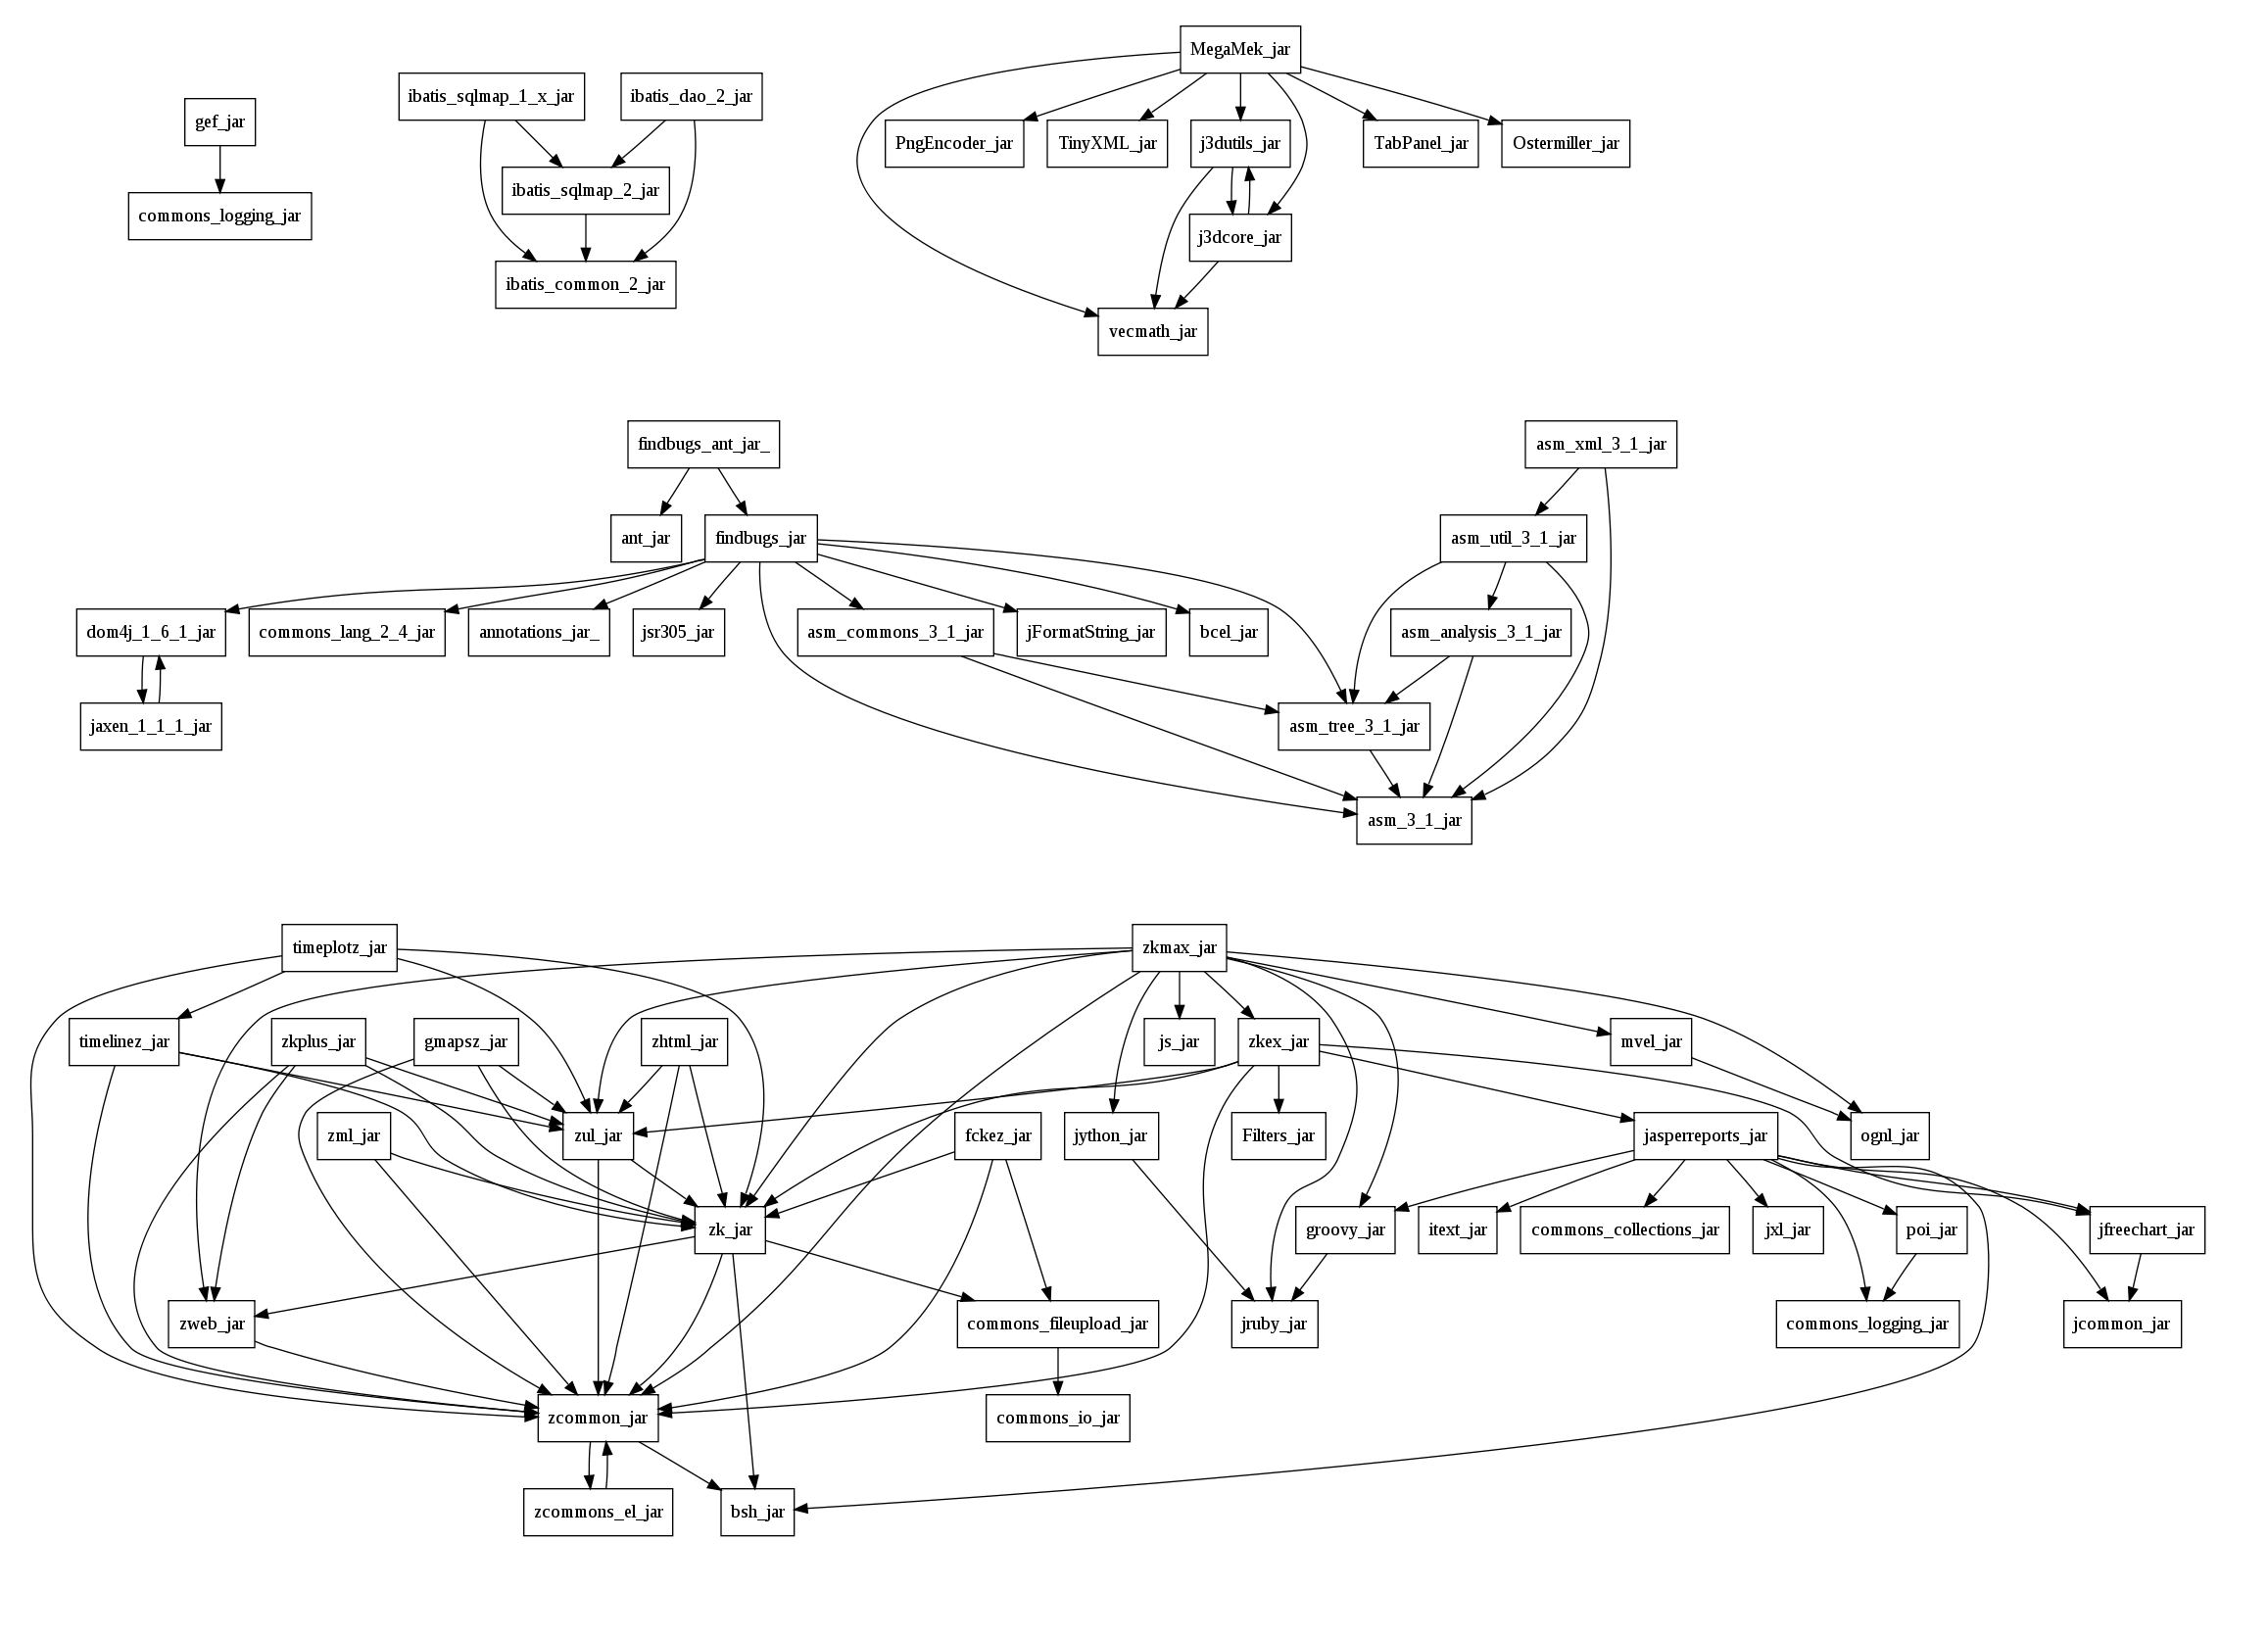
\includegraphics[width=1.0\textwidth]{architectures}
\caption{Module dependency graphs}
\label{fig:architectures}
\end{figure*}

%02-gef
%04-ibatis
%08-megamek
%16-findbugs
%32-zk

The probabilities p, q and r were given all possible values from 0.0 up to 1.0,
in 0.2 steps, such as the sum of the probabilities was 1. Since the only events
that create vertices are those associated with probabilities p and q, we imposed
the additional restriction that p + q > 0.

For deltain and deltaout we assigned the integer numbers from 0 to 4. TODO: why

Finally, we chose mu from 0.0 to 0.6 in 0.2 steps. It does not make sense to
choose higher values since they mean that there will be more edges connecting
different modules.

In total, 9,500 networks were synthesized.

\subsection{LF networks}

Like BCR, we choose mu ranging from 0.0 to 0.6 in 0.2 steps. For the remaining
parameters we selected values from our sample of software systems. For degexp,
..., we picked the minimum, the median and the max values.

Total: 1,296 networks

\subsection{CGW networks}

We have varied each of the probabilities p1, p2, p3, and p4 from 0.0 to 1.0, in
0.2 steps, with $p1 > 0$ and $p1 + p2 + p3 + p4 = 1$. Each of the parameters
$e1$, $e2$, $e3$, and $e4$ assumed the values 1, 2, 4, and 8.

% We have imposed
%the additional restriction that $2 \cdot p4\cdot e4 \ge p1 \cdot e1 + p2\cdot e2$, 
%so the number of edges created is at least twice the number of edges removed
%(otherwise 
% TODO: DOES NOT MAKE SENSE

alpha in -1, 0, 1, 10, 100, 1000. 
m in 2, 4, 8, 16, 32 (just like bcr and lfr)

In total, 38,790 networks were synthesized.

\subsection{Results}
% This subsection needn't to be big. It's just numbers.

We used our classifier ...

Table: Model | Number of Networks | Realistic Networks | Percent \%

Show some graphs: histogram of average correlations for each model.
\ref{fig:histograms}


\begin{figure*}[!t]
\center

\subfigure[Software network]{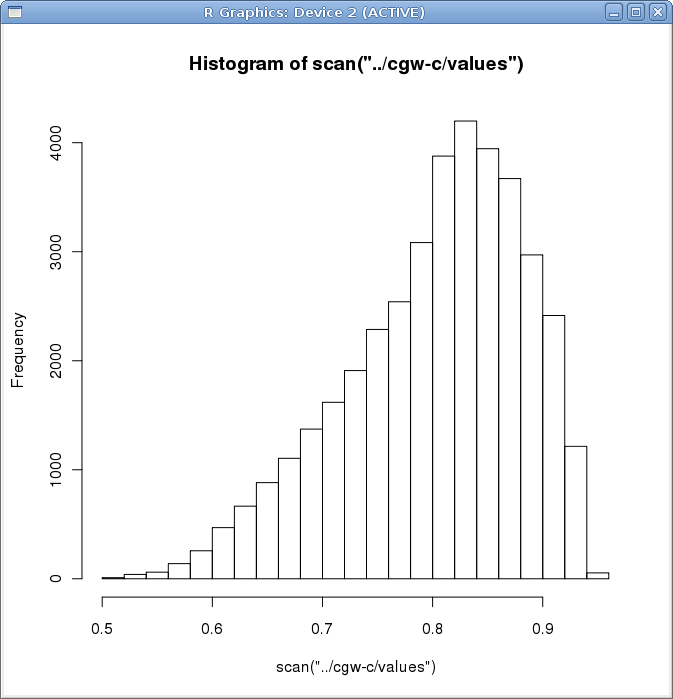
\includegraphics[width=1.0in]{hist-cgw}}

\subfigure[Non-software network]{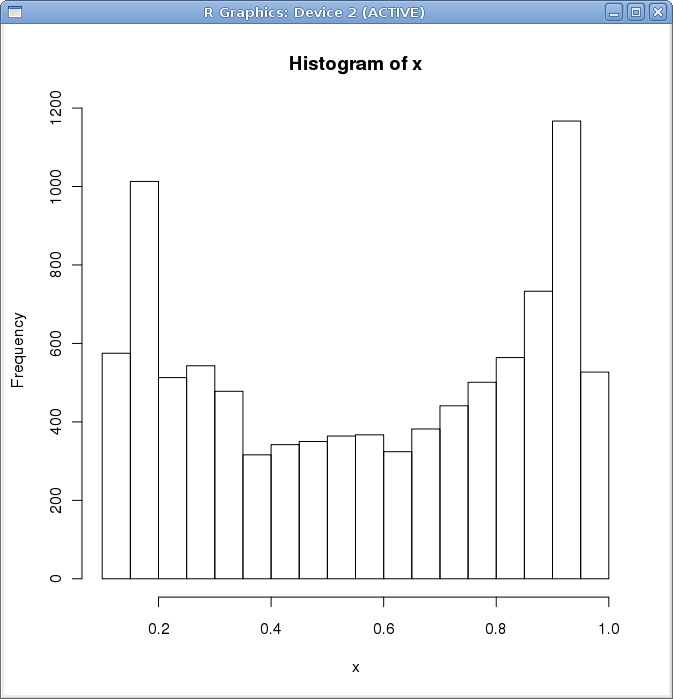
\includegraphics[width=1.0in]{hist-bcr}}

\subfigure[Non-software network]{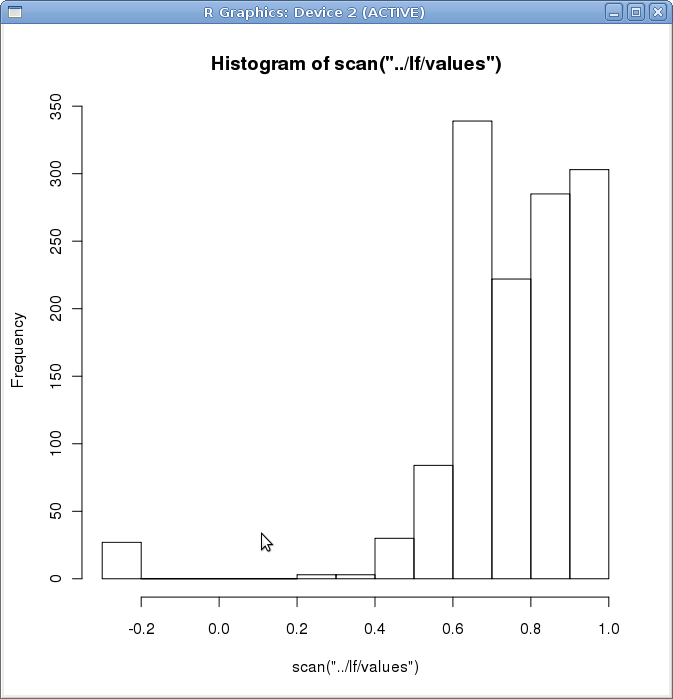
\includegraphics[width=1.0in]{hist-lf}}

\caption{Triad profiles}
\label{fig:histograms}
\end{figure*}

All models produce networks that resemble software networks.  For some
parameters, though, the networks are not realistic.

\subsection{Patterns in Parameters}

1R

Naive Bayes

\subsection{Homogeinity}

Pick realistic networks from a model. Are they similar to each other? (see
standard deviation) In other words: do the parameters make a difference?

Are they similar to networks generated by the other models? In other words: are
the models equivalent?

\section{Threats to validity}

% External validity (EV): can it be generalized?
Structural information isn't enough for a expert do produce a
decomposition (s/he may use data such as names and external documentation). 

Even when considering only structural information, is it true
that experts would find a decomposition similar to the reference decomposition
imposed by the model?

We generated only one network for each set of parameters. (as we've shown, some
parameters are redundant as they do not change significantly the realism)

Some clustering algorithms use weights and they weren't studied here.

EV: We've only studied 65 systems, which is not that much.

We only studied object-oriented systems implemented in Java. Maybe the results
would be different if we studied systems implement in other languagens or using
other paradigms. The choice of a particular technique for extracting
dependencies (static analysis) may also have impact on the structure of the
networks.

% Koschke says that experts decompositions vary by no more than 80? percent.

\section{Conclusion and Future Work}
% revised 2009-09-03

We have shown empirically that network models found in the literature can
synthesize networks that resemble the network of dependencies between classes in
object-oriented systems. This result supports the use of synthetic networks in
the evaluation of software clustering algorithms.
%that operate on class dependency networks. 

The use of synthetic data is common in distributed computing research, but still
underexplored in software engineering research. Because many reverse engineering
tasks rely on dependency data, we expect this work to have impact beyond the
software clustering community.

%Although the use of models and synthetic data is somewhat common in distributed
%computing research, it is underexplored in software engineering research. We
%expect this work to contribute to explore t
%common in distributed computing research, simulation is underexplored
%in software engineering. This work opens a door to the usage of simulation in
%the field of reverse engineering of software in order to evaluate RE 
%algorithms.

We accept that it is important to evaluate the algorithms with real software
networks, but we argue that the use of synthetic networks in a complementary
manner can give researchers new insights about the algorithms. First, the use of
models allows the creation of large test sets, thus diminishing the small sample
effects. Moreover, the networks are created in a controlled way, according to
model parameters, so it is possible to study the behavior of the algorithms with
different parameter values.

In a future work, we intend to use synthetic networks in the evaluation of
software clustering algorithms that were previously studied with real networks
\cite{Wu2005}. After that we will be able to compare the results obtained by
both approaches.

\section{Appendix A: list of networks}

TODO: Show as Table: Name, Vertices, Edges

Software networks:

From SourceForge:
AbaGuiBuilder-1.8
alfresco-labs-deployment-3Stable
aoi272
stendhal-0.74
battlefieldjava-0.1
checkstyle-5.0
dom4j-1.6.1
findbugs-1.3.8
freetts-1.2.2-bin
ganttproject-2.0.9
geoserver-2.0-beta1-bin
geotools-2.5.5-bin
gfp\_0.8.1
hibernate-distribution-3.3.1.GA-dist
hsqldb\_1\_8\_0\_10
iBATIS\_DBL-2.1.5.582
iReport-nb-3.5.1
JabRef-2.5b2-src
jailer\_2.9.9
jalopy-1.5rc3
jasperreports-3.5.2-project
jfreechart-1.0.13
pentaho-reporting-engine-classic-0.8.9.11
jGnash-2.2.0
jgraphpad-5.10.0.2
jmsn-0.9.9b2
juel-2.1.2
JXv3.2rc2deploy
makagiga-3.4
MegaMek-v0.34.3
iFreeBudget-2.0.9
mondrian-3.1.1.12687
oddjob-0.26.0
openxava-3.1.2
pdfsam-1.1.3-out
pjirc\_2\_2\_1\_bin
pmd-bin-4.2.5
proguard4.3
smc\_6\_0\_0
squirrel-sql-3.0.1-base
squirrel-sql-3.0.1-standard
tvbrowser-2.7.3-bin
villonanny-2.3.0.b02.bin
rapidminer-4.4-community
zk-bin-3.6.1

From other places:

ArgoUML-0.28
GEF-0.13-bin
Hl7Comm.1.0.1
IRPF2009v1.1
broker-4.1.5
dbwrench
ec2-api-tools
ermodeller-1.9.2-binary
flyingsaucer-R8
gdata-src.java-1.31.1
guice-2.0
gwt-windows-1.6.4
jai-1\_1\_4-pre-dr-b03-lib-linux-i586-08\_Jun\_2009
jakarta-tomcat-5.0.28-embed
juxy-0.8
myjgui\_0.6.6
peer-4.1.5
subethasmtp-3.1
thinkui\_sqlclient-1.1.2
worker-4.1.5

Other networks:

3 circuit networks (circuit-s208 circuit-s420 circuit-s838)

5 facebook networks (facebook-Caltech36 facebook-Georgetown facebook-Oklahoma
facebook-Princeton facebook-UNC28)

5 language networks (lang-english  lang-french lang-japanese lang-spanish)

43 metabolic networks

3 protein networks (protein-a4j protein-AOR protein-eaw)

2 social networks (social-leader social-prison)

other networks:

polblogs

yeast

beta3sreduced
celegansneural

czech
ecoli-metabolic
